\documentclass{article}
\usepackage{prepa}

\usetikzlibrary{arrows.meta,positioning,shapes,decorations.markings}

\title{Correction}
\author{}
\date{}

\begin{document}

\maketitle

\section*{Exercice 1}

\subsection*{Question 1}
    $f\in [20 Hz ; 20 kHz]$

\subsection{Question 2}
Ces fréquences correspondent à des longueurs d'ondes

$\lambda = \frac{c}{f} = \frac{3 \times 10^8}{20} \simeq \SI{15000}{km}$ (pour \SI{20}{Hz})

$\lambda = \frac{3 \times 10^8}{20 \times 10^3} \simeq \SI{15}{km}$ (pour \SI{20}{kHz})

Il faudrait une antenne de \SI{15000}{km} !

\subsection*{Question 3}

$$v_s = v_p(t) + k v_e(t) v_p(t)$$

\subsection*{Question 4}

$$v_s = A_p \cos(2\pi f_p t) + k A_p \cos(2\pi f_p t) A_e \cos(2\pi f_e t)$$

$$= A_p \cos(2\pi f_p t) \left[1 + k A_e \cos(2\pi f_e t)\right]$$

\textbf{2 cas :}

\begin{minipage}{0.45\textwidth}
\textbf{Si} $k A_e < 1$ (signal non surmodulé) \\
$1 + k A_e \cos(2\pi f_e t)$ est toujours positif
\begin{center}
    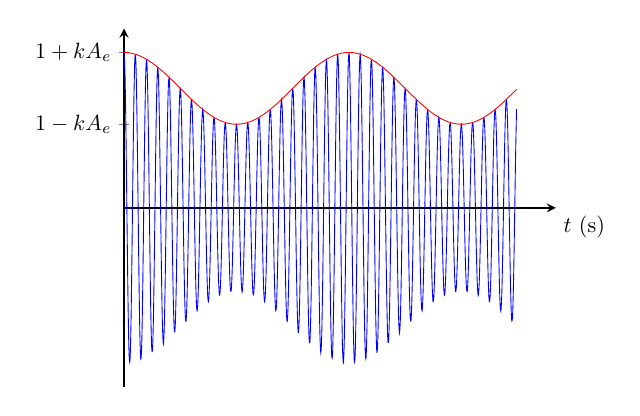
\begin{tikzpicture}[scale=0.8]  
      \begin{axis}[
          ymin=-1.5, ymax=1.5,
          xmin=0, xmax=11,
          %enlargelimits,
          axis x line=center,
          axis y line=center,
          xlabel={$t$ (s)},
          xlabel style={below right},
          %label style = {at={(ticklabel cs:1.1)}}
          axis line style=thick,
          ytick = {0.7,1.3},
          yticklabels={$1-kA_e$, $1+kA_e$},
          xtick = \empty,
        ]
        \addplot expression[samples=400,domain=0:10, mark=none, smooth] {cos(2*pi*200*x)*(1+0.3*cos(2*pi*10*x))};
        \addplot expression[samples=400,domain=0:10, mark=none, smooth, color=red] {1+0.3*cos(2*pi*10*x)};
      \end{axis}
    \end{tikzpicture}
\end{center}
\end{minipage}
\hfill
\begin{minipage}{0.45\textwidth}
\textbf{Si} $k A_e > 1$ (signal surmodulé)\\
$1 + k A_e \cos(2\pi f_e t)$ peut être négatif
\begin{center}
    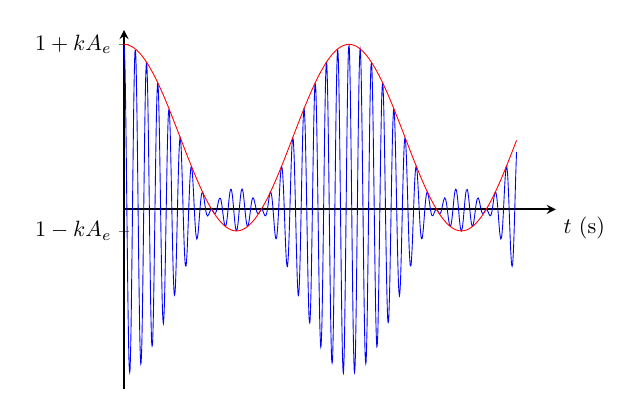
\begin{tikzpicture}[scale=0.8]
      \begin{axis}[
          ymin=-2.5, ymax=2.5,
          xmin=0, xmax=11,
          %enlargelimits,
          axis x line=center,
          axis y line=center,
          xlabel={$t$ (s)},
          xlabel style={below right},
          %label style = {at={(ticklabel cs:1.1)}}
          axis line style=thick,
          ytick = {-0.3,2.3},
          yticklabels={$1-kA_e$, $1+kA_e$},
          xtick = \empty,
        ]
        \addplot expression[samples=400,domain=0:10, mark=none, smooth] {cos(2*pi*200*x)*(1+1.3*cos(2*pi*10*x))};
        \addplot expression[samples=400,domain=0:10, mark=none, smooth, color=red] {1+1.3*cos(2*pi*10*x)};
      \end{axis}
    \end{tikzpicture}
\end{center}
\end{minipage}

On peut démoduler de façon non-ambigüe si $k < \frac{1}{A_e}$.

\subsection*{Question 5}

$$v_e(t) = A_p \cos(2\pi f_p t) + \frac{k A_e A_p}{2}\left[\cos(2\pi(f_p + f_e)t) + \cos(2\pi(f_p - f_e)t)\right]$$

\textbf{Spectre de} $V_S$ :
\begin{center}
\centering
\begin{tikzpicture}
\draw[->] (0,0) -- (8,0) node[right] {$f$};
\draw[->] (0,0) -- (0,3) node[above] {Amplitude};

% Raies spectrales
\draw[red, thick, ->] (2.5,0) --++ (0,2.5);
\draw[red, thick, ->] (1.5,0) --++ (0,1);
\draw[red, thick, ->] (3.5,0) --++ (0,1);

\node[left] at (0,2.5) {$A_p$};
\node[left] at (0,1) {$\frac{k A_e A_p}{2}$};

% Labels fréquences
\node[below] at (1.5,-0.5) {$f_p - f_e$};
\node[below] at (2.5,0) {$f_p$};
\node[below] at (3.5,-0.5) {$f_p + f_e$};
\end{tikzpicture}
\end{center}

\subsection*{Question 6}

Si $V_e$ a pour spectre :

\begin{center}
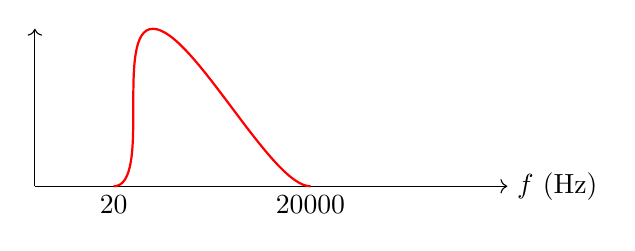
\begin{tikzpicture}
\draw[->] (0,0) -- (6,0) node[right] {$f$ (Hz)};
\draw[->] (0,0) -- (0,2);
\draw[red, thick] (1,0) .. controls (1.5,0) and (1,2) .. (1.5,2) .. controls (2,2) and (3,0) .. (3.5,0);
\node[below] at (1,0) {20};
\node[below] at (3.5,0) {20000};
\end{tikzpicture}
\end{center}

alors $V_s$ a pour spectre :

\begin{center}
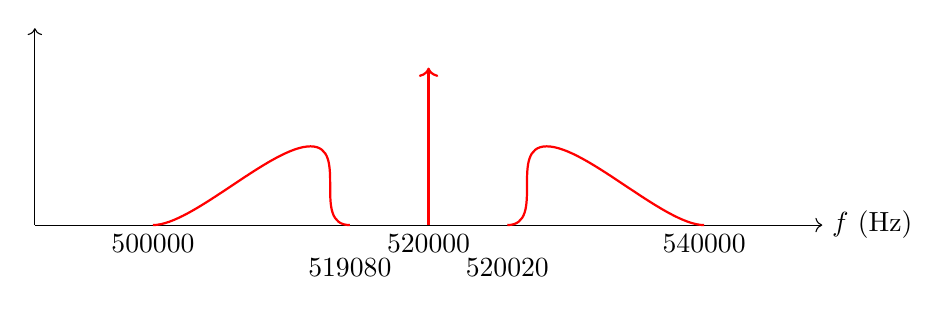
\begin{tikzpicture}
\draw[->] (0,0) -- (10,0) node[right] {$f$ (Hz)};
\draw[->] (0,0) -- (0,2.5);

% Bandes latérales
\draw[red, thick] (6,0) .. controls (6.5,0) and (6,1) .. (6.5,1) .. controls (7,1) and (8,0) .. (8.5,0);
\draw[red, thick] (4,0) .. controls (3.5,0) and (4,1) .. (3.5,1) .. controls (3,1) and (2,0) .. (1.5,0);

\draw[red, thick, ->] (5,0) -- (5,2);

% Labels
\node[below] at (1.5,0) {500000};
\node[below] at (5,0) {520000};
\node[below] at (8.5,0) {540000};
\node[below] at (4,-0.3) {519080};
\node[below] at (6,-0.3) {520020};
\end{tikzpicture}
\end{center}

\subsection*{Question 7}

Le spectre de $V_s$ occupe \SI{40}{kHz} sur le spectre.
Dans la bande $[520 ; 1620] \unit{kHz}$, on peut en faire tenir $\frac{1620 - 520}{40} \simeq 27$ canaux.

\section*{Exercice 2}

\subsection*{Question 1}

\begin{center}
  \begin{circuitikz}
    \draw (0,0) node[en amp] (ALI) {};
    \draw (ALI.+) --++ (0,-0.7) node[ground] {};
    \draw (ALI.-) --++ (0,2) to[R,l=$R$,v=$v_s-V_-$,i<=$i$] ++ (2.3,0) -| (ALI.out) --++ (0.5,0) node[right] {$v_s$};
    \draw (ALI.-) --++ (-1,0) to[R,l=$R_1$,v=$v_2-V_-$,i<=$i_2$] ++ (-2,0) node[left] {$v_2$};
    \draw (ALI.-) -|++ (-1,2) to[R,l=$R_2$,v=$v_1-V_-$,i<=$i_1$] ++ (-2,0) node[left] {$v_1$};
  \end{circuitikz}
\end{center}

\textbf{Kirchhoff's law :} $i_1 + i_2 + i + i_- = 0$

But $i' \simeq 0$ so $i_1 + i_2 + i = 0$

$\Rightarrow \frac{1}{R_1}(v_1 - V_-) + \frac{1}{R_2}(v_2 - V_-) + \frac{1}{R}(v_s - V_-) = 0$

$\Rightarrow V_-\left(\frac{1}{R_1} + \frac{1}{R_2} + \frac{1}{R}\right) = \frac{v_1}{R_1} + \frac{v_2}{R_2} + \frac{v_s}{R}$

$$V_- = \frac{\frac{v_1}{R_1} + \frac{v_2}{R_2} + \frac{v_s}{R}}{\frac{1}{R_1} + \frac{1}{R_2} + \frac{1}{R}}$$

\subsection*{Question 2}

ILA idéal et rétroaction négative $\Rightarrow \epsilon = 0$

$\Rightarrow V_- = V_+ = 0$

$\Rightarrow \frac{v_1}{R_1} + \frac{v_2}{R_2} + \frac{v_s}{R} = 0$

$$v_s = -R\left(\frac{v_1}{R_1} + \frac{v_2}{R_2}\right)$$

\subsection*{Question 3}

If $R = R_1 = R_2$ : $v_s = -v_1 - v_2$

\subsection*{Question 4}

$H_2 = \frac{v_{S,2}}{v_s} = \frac{v_1 + v_2}{-v_1 - v_2} = -1$

An inverting amplifier can have this transfer function:

$H_2 = -\frac{R_3}{R_4} \Rightarrow \text{if } R_3 = R_4 \Rightarrow H_2 = -1$

\begin{center}
\centering
\begin{circuitikz}
  \draw (0,0) node[en amp] (ALI) {};
  \draw (ALI.+) --++ (0,-0.7) node[ground] {};
  \draw (ALI.-) --++ (0,1.5) to[R,l=$R_3$] ++ (2.3,0) -| (ALI.out);
  \draw (ALI.-) --++ (-1,0) to[R,l=$R_3$] ++ (-2,0);
\end{circuitikz}
\end{center}

\section*{Exercice 3}

\subsection*{Question 1}

$$s_{AM}(t) = A_p \cos(2\pi f_p t)(1 + k s(t))$$
$$s_p(t) = A_p \cos(2\pi f_p t)$$
$$s_i(t) = A_p^2 \cos^2(2\pi f_p t)(1 + k s(t))$$

\begin{center}
\begin{tikzpicture}
\draw[->] (0,0) -- (10,0) node[right] {$f (\unit{kHz})$};
\draw[->] (0,0) -- (0,2.5) node[right] {spectre du signal original};
\draw[red, thick] (0,0) .. controls (0.5,0) and (0,1) .. (0.5,1) .. controls (1,1) and (1,0) .. (1.5,0);
\node[below] at (0,0) {$0$};
\node[below] at (1.5,0) {$10$};
\end{tikzpicture}

\begin{tikzpicture}
\draw[->] (0,0) -- (10,0) node[right] {$f (\unit{kHz})$};
\draw[->] (0,0) -- (0,2.5) node[right] {spectre de $s_p$};
\draw[red, thick, ->] (4,0) -- (4,2);
\node[below] at (0,0) {$0$};
\node[below] at (4,0) {$200$};
\end{tikzpicture}

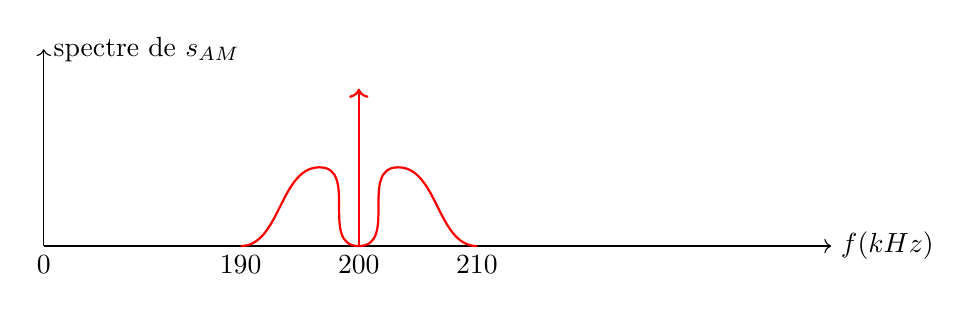
\begin{tikzpicture}
\draw[->] (0,0) -- (10,0) node[right] {$f (\unit{kHz})$};
\draw[->] (0,0) -- (0,2.5) node[right] {spectre de $s_{AM}$};
\draw[red, thick, ->] (4,0) -- (4,2);
\begin{scope}[xshift=4cm]
  \draw[red, thick] (0,0) .. controls (0.5,0) and (0,1) .. (0.5,1) .. controls (1,1) and (1,0) .. (1.5,0);
  \node[below] at (1.5,0) {$210$};
\end{scope}
\begin{scope}[xscale=-1,xshift=-4cm]
  \draw[red, thick] (0,0) .. controls (0.5,0) and (0,1) .. (0.5,1) .. controls (1,1) and (1,0) .. (1.5,0);
\end{scope}
\node[below] at (2.5,0) {$190$};
\node[below] at (0,0) {$0$};
\node[below] at (4,0) {$200$};
\end{tikzpicture}

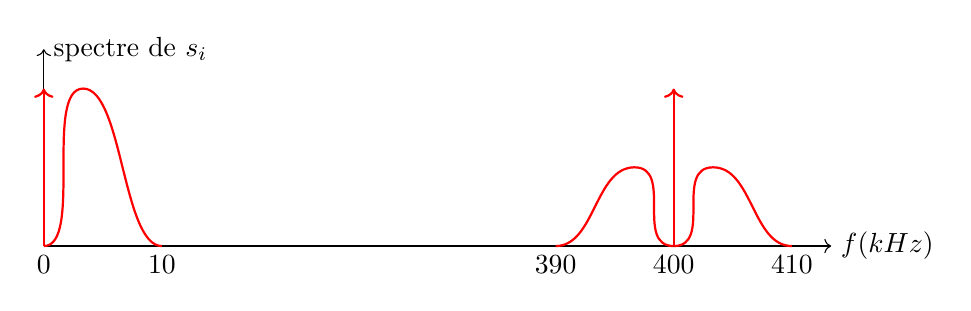
\begin{tikzpicture}
\draw[->] (0,0) -- (10,0) node[right] {$f (\unit{kHz})$};
\draw[->] (0,0) -- (0,2.5) node[right] {spectre de $s_i$};
\draw[red, thick, ->] (8,0) --++ (0,2);
\draw[red, thick, ->] (0,0) --++ (0,2);
\begin{scope}[yscale=2]
  \draw[red, thick] (0,0) .. controls (0.5,0) and (0,1) .. (0.5,1) .. controls (1,1) and (1,0) .. (1.5,0);
  \node[below] at (1.5,0) {$10$};
\end{scope}
\begin{scope}[xshift=8cm]
  \draw[red, thick] (0,0) .. controls (0.5,0) and (0,1) .. (0.5,1) .. controls (1,1) and (1,0) .. (1.5,0);
  \node[below] at (1.5,0) {$410$};
\end{scope}
\begin{scope}[xscale=-1,xshift=-8cm]
  \draw[red, thick] (0,0) .. controls (0.5,0) and (0,1) .. (0.5,1) .. controls (1,1) and (1,0) .. (1.5,0);
\end{scope}
\node[below] at (6.5,0) {$390$};
\node[below] at (0,0) {$0$};
\node[below] at (8,0) {$400$};
\end{tikzpicture}

\begin{tikzpicture}
\draw[->] (0,0) -- (10,0) node[right] {$f (\unit{kHz})$};
\draw[->] (0,0) -- (0,2.5) node[right] {spectre de $s$};
\draw[red, thick, ->] (0,0) --++ (0,2);
\draw[red, thick] (0,0) .. controls (0.5,0) and (0,1) .. (0.5,1) .. controls (1,1) and (1,0) .. (1.5,0);
\node[below] at (0,0) {$0$};
\node[below] at (1.5,0) {$10$};
\end{tikzpicture}
\end{center}

\subsection*{Question 2}

On peut prendre $f_c = \SI{16}{kHz} = \frac{1}{2\pi RC}$

avec par exemple $R = \SI{1}{k\ohm}$ et $C = \SI{10}{nF}$

\section*{Exercice 4}

\subsection*{Question 1}

\begin{center}
\centering
\begin{circuitikz}
\draw (0,0) to[ncs] (2,0) to[R, l_=$R$] (2,-2) -- (0,-2) to[open,v=$e$] (0,0);
\draw (2,0) -- (3,0) to[C, l_=$C$,v^<=$s$] (3,-2) -- (2,-2);
\end{circuitikz}
\end{center}

$$s(t) = e(t)$$

\subsection*{Question 2}

\begin{center}
\centering
\begin{circuitikz}
\draw (0,0) to[nos,i=$i$] (2,0) to[R, l_=$R$,i=$i_1$] (2,-2) -- (0,-2) to[open] (0,0);
\draw (2,0) -- (3,0) to[C, l_=$C$,v^<=$s$,i=$i_2$] (3,-2) -- (2,-2);
\end{circuitikz}
\end{center}

On a $0=i= i_1+i_2$ donc $i_1 = -i_2$ d'où $\frac{s}{R} = -C\frac{ds}{dt}$ donc $$\frac{ds}{dt} + \frac{1}{RC}s = 0$$

\subsection*{Question 3}

Code Capytale : \texttt{2acf-7216571}

\subsection*{Question 4}

Le signal $1$ est démodulé correctement, contrairement au $2$.

\section*{Exercice 5}

\begin{center}
    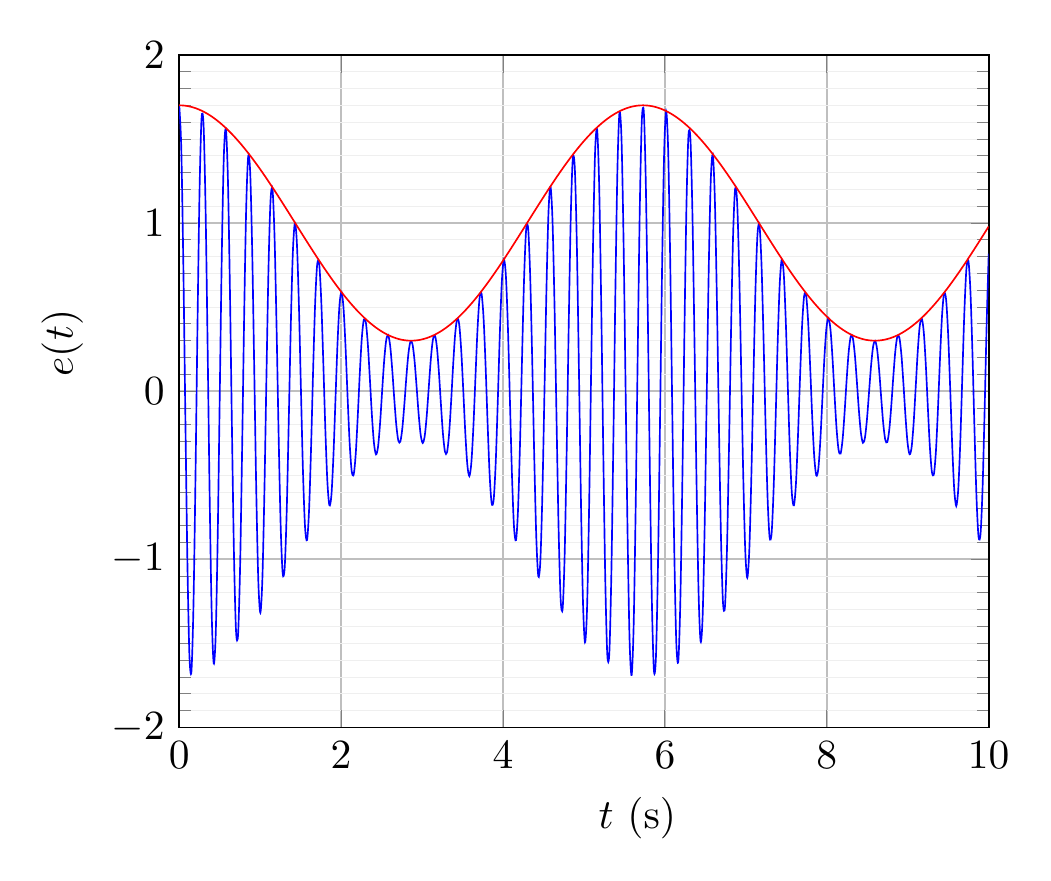
\begin{tikzpicture}[scale=1.5]
      \begin{axis}[
          ymin=-2, ymax=2,
          xmin=0, xmax=10,
          %enlargelimits=true,
          xlabel={$t$ (s)},
          xlabel style={below right},
          ylabel={$e(t)$},
          ylabel style={above right},
          %label style = {at={(ticklabel cs:1.1)}}
          grid=both,
          minor grid style={very thin, lightgray!25}, 
          major grid style={thin},
          minor y tick num=9,
        ]
        \addplot expression[samples=400,domain=0:10, mark=none, smooth] {cos(2*pi*200*x)*(1+0.7*cos(2*pi*10*x))};
        \addplot expression[samples=400,domain=0:10, mark=none, smooth,color=red] {(1+0.7*cos(2*pi*10*x))};
      \end{axis}
    \end{tikzpicture}
\end{center}

La modulante a pour valeur max $(1+kA)=1.7$ et pour valeur min $(1-kA)=0.3$. On en déduit $2kA=1.7-0.3=1.4$ d'où le taux de modulation $kA=0.7$.

\section*{Exercice 6}

subsection*{Question 1}
$i$


\section*{Exercice 7}
Pour envoyer pleusieurs stations de radio en même temps sur les onde, on utilise une technique appelée modulation. Le principe, c'est de mélanger la station de radio qu'on veut émettre à un autre signal, qu'on appelle la porteuse (car c'est elle qui <<transporte>> la station de radio). À chaque station de radio correspond sa porteuse.

Pour <<décoder>> la radio (on dit <<démoduler>>), le poste de radio mélange à son tour le signal reçu avec la porteuse de la station qu'on veut écouter (la même qu'on avait utilisé pour moduler) et, après un peu de filtrage pour enlever les signaux indésirables, on retrouve avec le signal de la station qu'on souhaite écouter.

Il faut juste faire attention que plusieurs stations n'aient pas des porteuses trop proches, sinon ils risqueraient de se mélanger et le poste de radio n'arriverait plus à les séparer. C'est ça qui limite le nombre de stations de radios qui peuvent être diffusées en même temps.

\end{document}